\section{Installazione ed avvio di SSD}
Per installare ed avviare l'applicazione \gloman{SSD} bisogna effettuare passi diversi in base al sistema operativo. Le varie versioni possono essere scaricate dal link: \newline{}
\centerline{\url{https://github.com/MercurySeven/project-SSD/releases}}

\subsection{Windows}
\begin{itemize}
\item \textbf{Scaricare:} cliccare sull'apposito link e scaricare il file denominato \textit{SSD.exe};
\item \textbf{Avviare l'applicazione:} cliccare sull'applicazione appena scaricata.
\end{itemize}

\subsection{MacOS}
\begin{itemize}
\item \textbf{Scaricare:} cliccare sull'apposito link e scaricare il file denominato \textit{SSD\_macOS.zip};
\item \textbf{Avviare l'applicazione:} decomprimere il file, aprire la cartella, dare i permessi di esecuzione allo script launch.sh e avviarlo da terminale.
\end{itemize}
\begin{figure}[H]
    \centering
    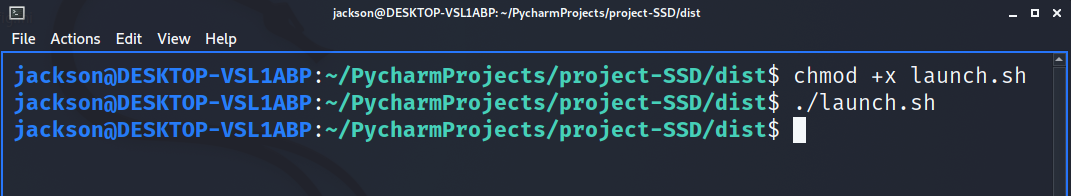
\includegraphics[scale = 0.3]{components/img/permessi-eseguire-ed-eseguire-launch.png}
    \caption{Dare i permessi ed eseguire launch.sh}
    \label{fig:Dare i permessi ed eseguire launch.sh}
\end{figure}

\subsection{Linux}
\begin{itemize}
\item \textbf{Scaricare:} cliccare sull'apposito link e scaricare il file denominato \textit{SSD.AppImage};
\item \textbf{Avviare l'applicazione:} cliccare sull'applicazione appena scaricata.
\end{itemize}

